
%(BEGIN_QUESTION)

Hva menes med følgende begreper:

\begin{itemize}
\item Prosessvariabel
\item ProsessVerdi PV 
\item Manipulerende Variabel MV
\item Pådrag 
%\item Forstyrrelse 
\item Avviket e 
\end{itemize}

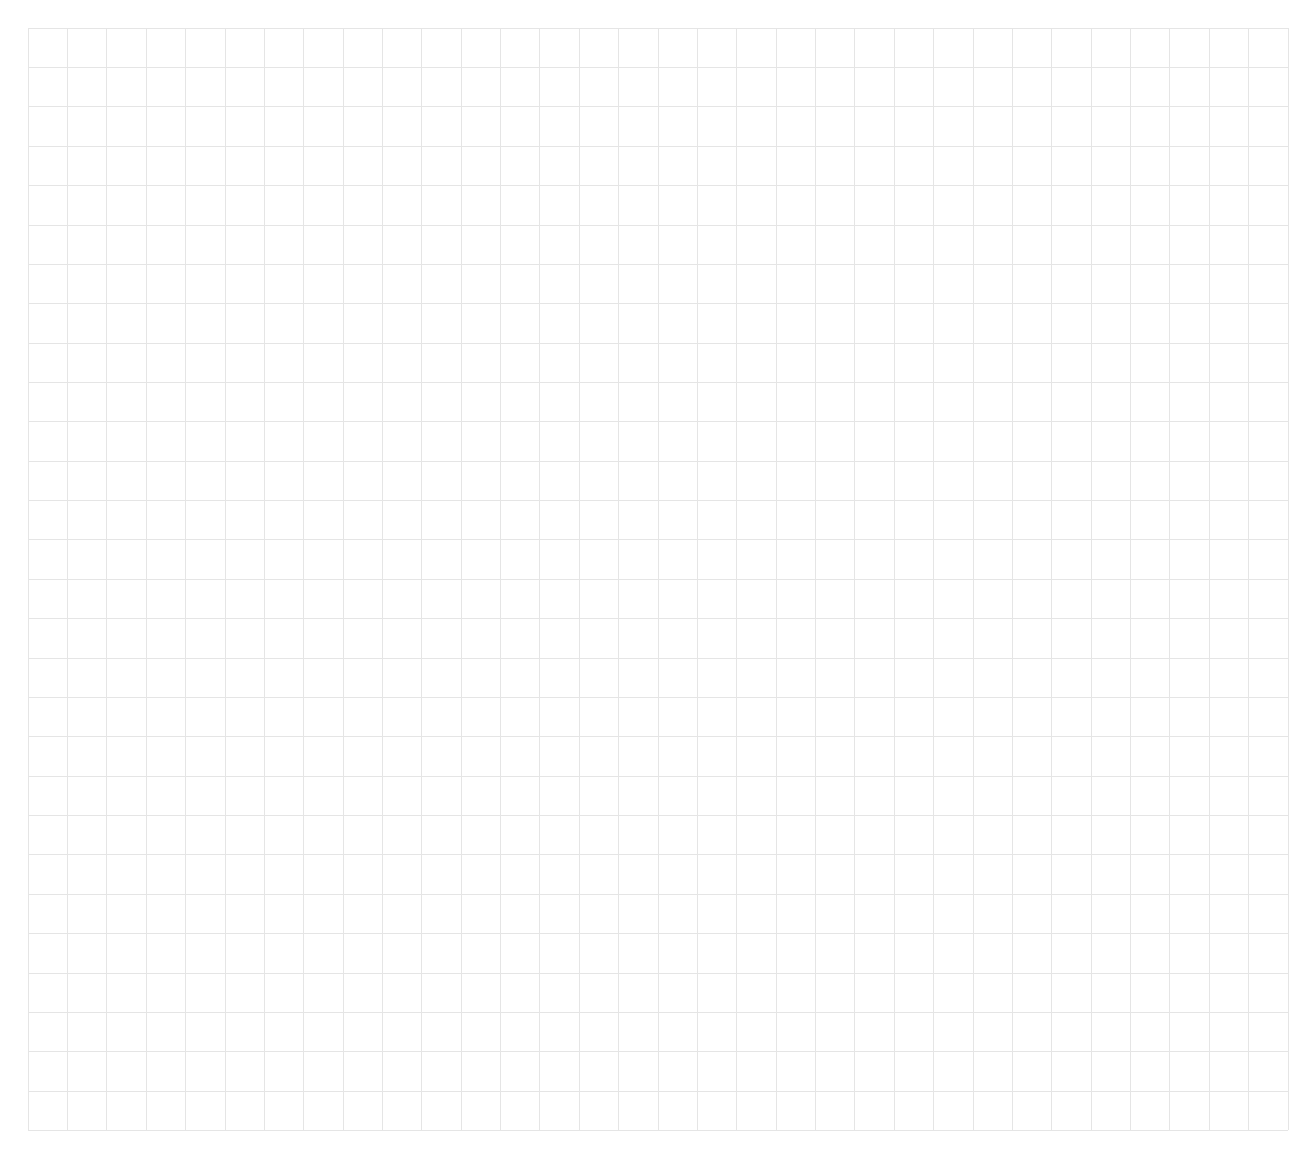
\begin{tikzpicture}
	\draw[step=0.5cm,gray!20,very thin]  grid (16,14) ;
\end{tikzpicture}

\vfil

\eject
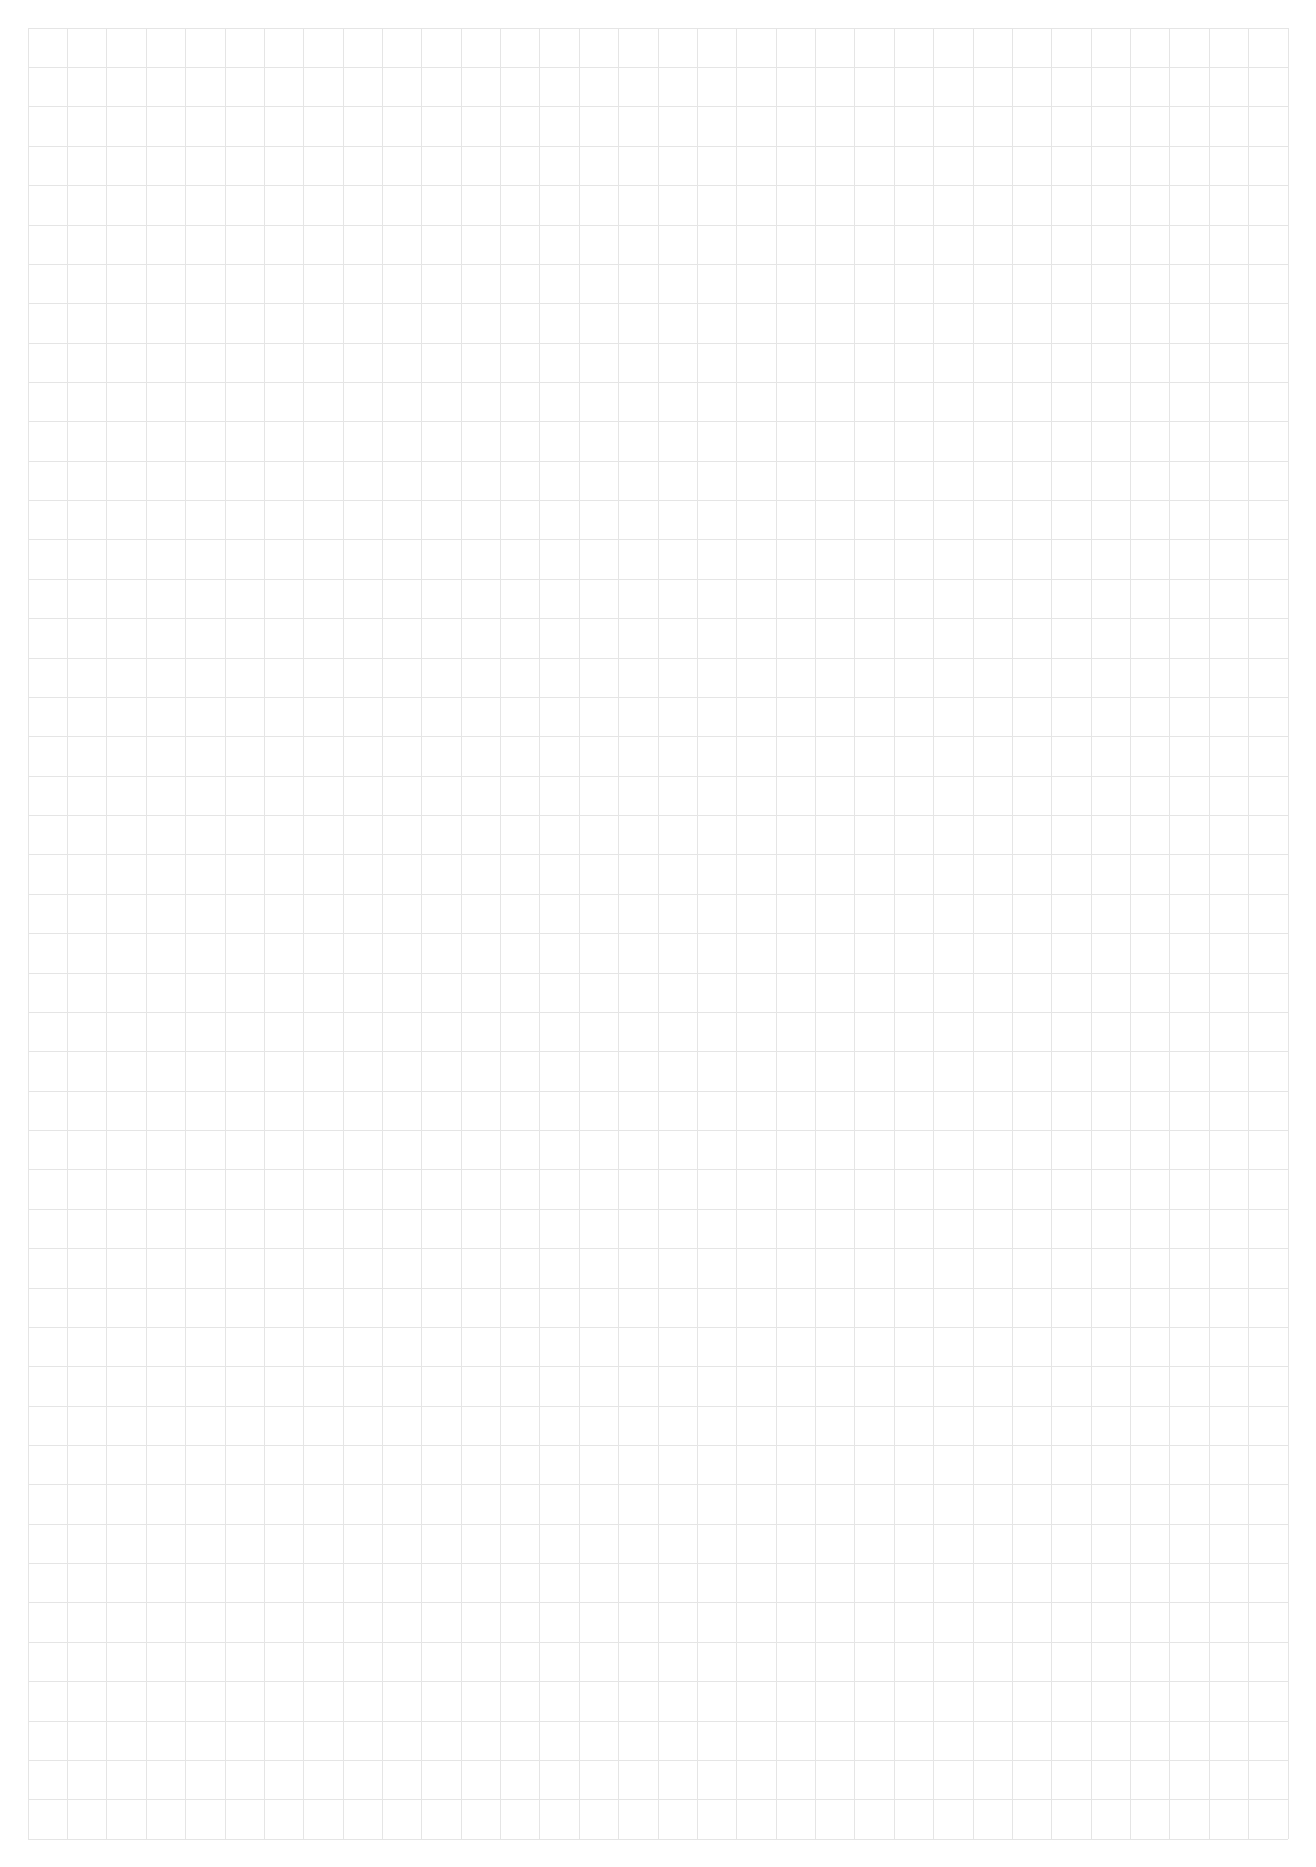
\begin{tikzpicture}
	\draw[step=0.5cm,gray!20,very thin]  grid (16,23) ;
\end{tikzpicture}
%\underbar{file i00000}
%(END_QUESTION)





%(BEGIN_ANSWER)

\begin{itemize}
%\item Regulator - En enhet som har til oppgave å påvirke prosessen slik at den oppnår en ønsket tilstand (f.eks. et ønsket nivå eller en ønsket temperatur).
%\item Prosess - Det anlegget eller systemet som inngår i reguleringen.
\item Prosessvariabel - Den fysiske størrelsen i prosessen som skal reguleres (nivå, trykk, temperatur etc.)
\item ProsessVerdi PV - Den verdien prosessvariabelen til enhver tid har.
%\item Settpunkt SP - Den verdien vi ønsker at prosessvariabelen skal ha.
\item Manipulerende Variabel MV - Signalet som styrer pådragsorganet
%\item Forsyning - 
\item Pådrag - Det som er ment å variere prosessvariabelen. F.eks. væske inn i en nivåtank. 
%\item Belastning - Det som tas ut av prosessen ved konstant PV. Vil ha sammeverdi som pådraget. 
%\item Forstyrrelse - Forandringer som påvirker verdien til prosessvariabelen. 
\item Avviket e - Forskjellen mellom PV og SP (Direkte virkning PV-SP, Reverserende virkning SP-PV)
%\item Pådragsorgan - Den komponenten som styrer pådraget (f.eks. motoren
%i bilen som påvirker hastigheten, eller ventilen som påvirker nivået
%i tanken).
%\item Forstillingsenhet - I vårt eksempel med regulering av bilens hastighet,
%er forstillingsenheten forgasseren. Motoren er pådragsorganet i reguleringssløyfen.
%\item Auto og Manuell modus (Lukket- eller åpensløyfe). Om pådraget styres
%av regulatoren eller en manuell innstilt verdi. 
%\item LRV og URV ( Lover Range Value og Upper Range value, Laveste og høyeste
%verdi målesignalet kan ha.)
\end{itemize}

%(END_ANSWER)





%(BEGIN_NOTES)


%INDEX% Control, Definitions: (word or phrase here)

%(END_NOTES)


